% !TEX TS-program = pdflatex
% !TEX encoding = UTF-8 Unicode

\documentclass[a4paper, titlepage=false, parskip=full-, 10pt]{scrartcl}

\usepackage[utf8]{inputenc}
\usepackage[T1]{fontenc}
\usepackage[english, ngerman]{babel}
\usepackage{babelbib}
\usepackage{hyperref}
\usepackage{listings}
\usepackage{framed}
\usepackage{color}
\usepackage{graphicx}
\usepackage[normalem]{ulem}
\usepackage{cancel}
\usepackage{array}
\usepackage{amsmath}
\usepackage{amssymb}
\usepackage{amsthm}
\usepackage{algorithm}
\usepackage{algorithmic}
\usepackage{geometry}
\usepackage{subfigure}
\geometry{a4paper, top=20mm, left=35mm, right=25mm, bottom=40mm}

\newcounter{tasknbr}
\setcounter{tasknbr}{1}
\newenvironment{task}[1]{{\bf Aufgabe \arabic {tasknbr}\stepcounter{tasknbr}} (#1):\begin{enumerate}}{\end{enumerate}}
\newcommand{\subtask}[1]{\item[#1)]}

% Listings -----------------------------------------------------------------------------
\definecolor{red}{rgb}{.8,.1,.2}
\definecolor{blue}{rgb}{.2,.3,.7}
\definecolor{lightyellow}{rgb}{1.,1.,.97}
\definecolor{gray}{rgb}{.7,.7,.7}
\definecolor{darkgreen}{rgb}{0,.5,.1}
\definecolor{darkyellow}{rgb}{1.,.7,.3}
\lstloadlanguages{C++,[Objective]C,Java}
\lstset{
escapeinside={§§}{§§},
basicstyle=\ttfamily\footnotesize\mdseries,
columns=fullflexible,
keywordstyle=\bfseries\color{blue},
commentstyle=\color{darkgreen},      
stringstyle=\color{red},
numbers=left,
numberstyle=\ttfamily\scriptsize\color{gray},
breaklines=true,
showstringspaces=false,
tabsize=4,
captionpos=b,
float=htb,
frame=tb,
frameshape={RYR}{y}{y}{RYR},
rulecolor=\color{black},
xleftmargin=15pt,
xrightmargin=4pt,
aboveskip=\bigskipamount,
belowskip=\bigskipamount,
backgroundcolor=\color{lightyellow},
extendedchars=true,
belowcaptionskip=15pt}

%% Enter current values here: %%
\newcommand{\lecture}{Robotik WS15/16}
\newcommand{\tutor}{}
\newcommand{\assignmentnbr}{9}
\newcommand{\students}{Julius Auer, Thomas Tegethoff}
%%-------------------------------------%%

\begin{document}  
{\small \textsl{\lecture \hfill \tutor}}
\hrule
\begin{center}
\textbf{Übungsblatt \assignmentnbr}\\
[\bigskipamount]
{\small \students}
\end{center}
\hrule

\begin{task}{A*-Suche}
\item[]
Da die Geschwindigkeit des Autos sowie die Schrittweite fest aber beliebig sind, haben wir einen kontinuierlichen Zustandsraum und lassen die CLOSED-Liste weg. Für den hier behandelten einfachen Fall wäre eine Implementierung für kontinuierliche Zustandsräume ein unverhältnismäßig großer Aufwand.

Die Auswahl der Nachbarn eines Knotens ist straight-forward: Knoten repräsentieren eine 3D-Pose des Autos, so dass es stets 3 Nachbarn gibt - je nachdem, ob man links / rechts / gar nicht einlenkt. Die neue Pose für den neuen Knoten ergibt sich daraus direkt.

Interessant ist die Wahl einer guten Heuristik. Jeder Satz der Aufgabenstellung scheint hier laut {\bf Dubin} zu rufen - da hier etwas Einfacheres auch nicht ausreichend wäre (vor Allem die Bewegung in unmittelbarer Nähe eines Hindernisses erfordert hier ein Modell, das die nicht-Holonomie des Agenten abbilden kann), der Bedarf von etwas Ambitionierterem (Reeds-Shepp) aber durch die Randbedingungen der Aufgabe ausgeschlossen werden kann, implementieren wir als Heuristik eben genau besagte Dubin-Kurven.

Als einfache, wirkungsvolle Optimierung verbessern wir die Situation beim Rangieren vor einem Hindernis durch Hinzufügen eines Potentialfeld-ähnlichen Abstoßungseffektes: besonders ungünstig für die Wegfindung ist das frontale ''auf ein Hindernis zuhalten'', bei dem sich das Auto anschließend in langen Dubin-Kurven ''verheddern'' kann. Dies wiegt umso schwerer, wenn aufgrund der fehlenden CLOSED-Liste Kreise auftreten können. Als einfache Lösung wird einer Pose bei der ein Hindernis ''vor'' dem Auto ist ein zusätzliches Gewicht gegeben, das mit dem Abstand ($L_2$) zum Hindernis skaliert. Ist das Hindernis nicht direkt ''vor'' dem Auto darf dieser Effekt natürlich nicht auftreten, so dass man nach wie vor ''nah'' am Hindernis vorbeifahren kann.

Es seien im Folgenden: $e_p=2.5$ der zulässige Positionfehler, $e_o=1$ der zulässige Orientierungsfehler, $d$ die Schrittweite, $r=4$ der Radius des Wendekreises, $(x_o,y_o)\in\{\mathbb{R}^2|15\le x_o\le20\wedge -5\le y_o\le 20\}$ das Hindernis und $((x_t,y_t),(ox_t,oy_t))$ die Zielpose.

\newpage
\subtask{a}
$$((x_t,y_t),(ox_t,oy_t))=((6,3),(0,1))$$

\begin{figure}[!htpb]
\centering
\subfigure[$d=\pi$]{
  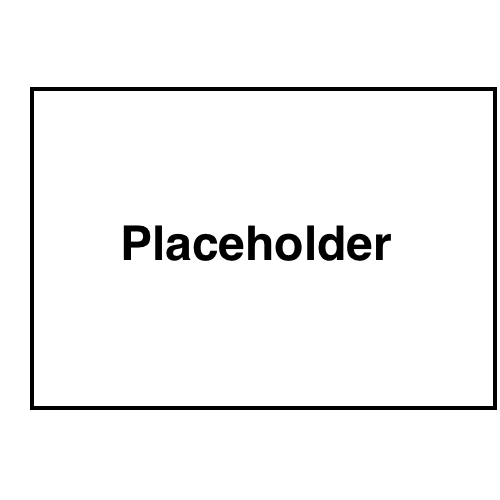
\includegraphics[width=0.48\linewidth]{platzhalter}
}
\subfigure[$d=\frac{\pi}{2}$]{
  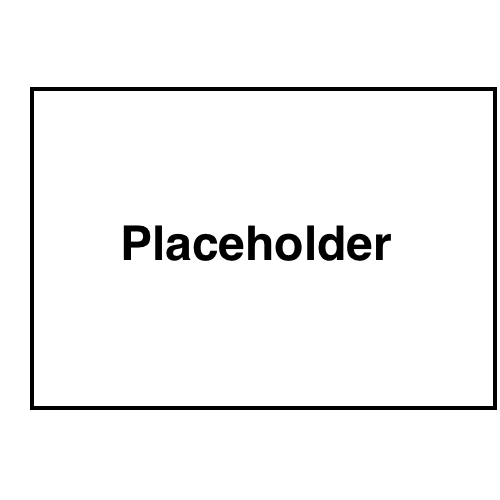
\includegraphics[width=0.48\linewidth]{platzhalter}
}
\caption{Plot a}
\end{figure}

\subtask{b}
$$((x_t,y_t),(ox_t,oy_t))=((0,5),(0,1))$$

\begin{figure}[!htpb]
\centering
\subfigure[$d=\pi$]{
  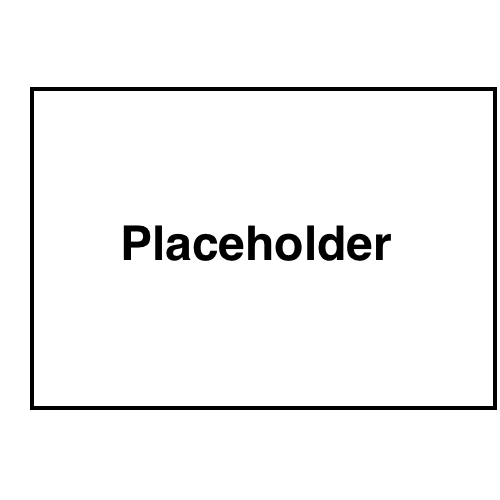
\includegraphics[width=0.48\linewidth]{platzhalter}
}
\subfigure[$d=\frac{\pi}{2}$]{
  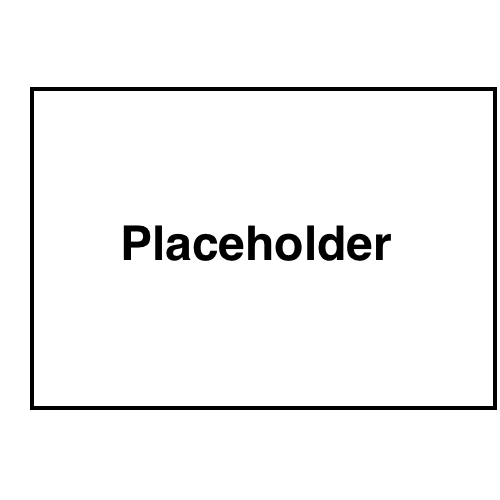
\includegraphics[width=0.48\linewidth]{platzhalter}
}
\caption{Plot b}
\end{figure}

\newpage
\subtask{c}
$$((x_t,y_t),(ox_t,oy_t))=((0,5),(1,0))$$

\begin{figure}[!htpb]
\centering
\subfigure[$d=\pi$]{
  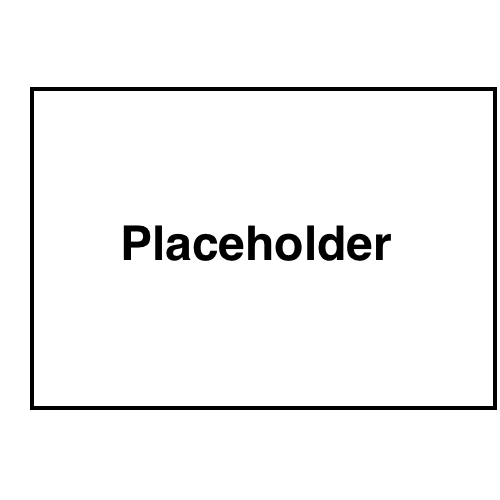
\includegraphics[width=0.48\linewidth]{platzhalter}
}
\subfigure[$d=\frac{\pi}{2}$]{
  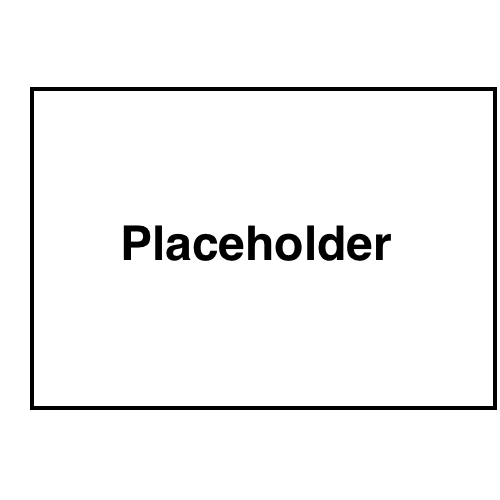
\includegraphics[width=0.48\linewidth]{platzhalter}
}
\caption{Plot c}
\end{figure}

\subtask{d}
$$((x_t,y_t),(ox_t,oy_t))=((30,15),(1,0))$$

\begin{figure}[!htpb]
\centering
\subfigure[$d=\pi$]{
  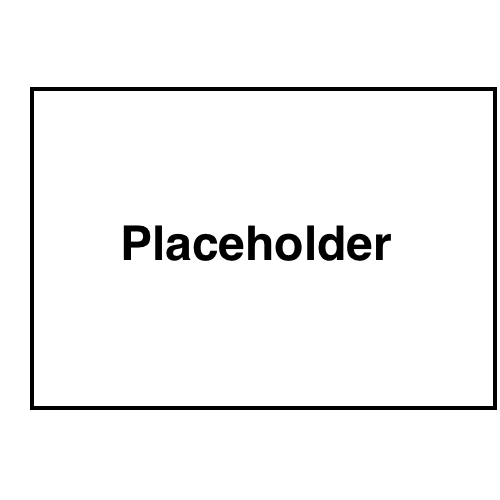
\includegraphics[width=0.48\linewidth]{platzhalter}
}
\subfigure[$d=\frac{\pi}{2}$]{
  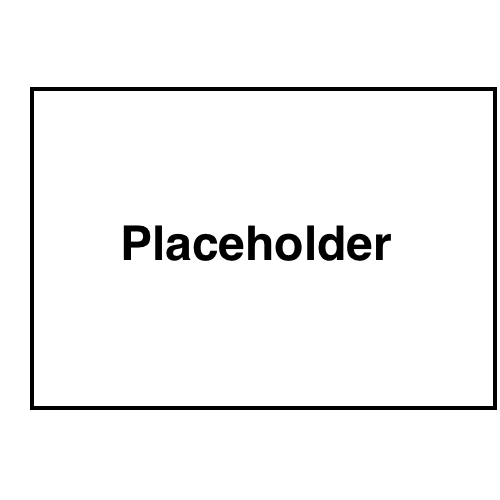
\includegraphics[width=0.48\linewidth]{platzhalter}
}
\caption{Plot d}
\end{figure}
\end{task}

\newpage
\begin{task}{}
\item[]
Der in Aufgabe 1 d) geschilderte Fall lässt sich in Abbildung \ref{fig:2-1} bewundern.

\begin{figure}[!htpb]
\centering
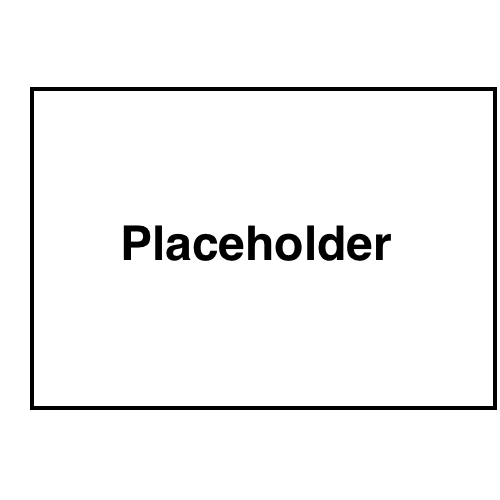
\includegraphics[width=0.8\linewidth]{platzhalter}
\caption{Pfad in rviz}
\label{fig:2-1}
\end{figure}
\end{task}
\end{document}